\documentclass[14pt,a4paper]{article}
\usepackage{txfonts}
\usepackage[utf8]{inputenc}
\usepackage[spanish]{babel}
\usepackage{amsmath}
\usepackage{amsfonts}
\usepackage{amssymb}
\usepackage{makeidx}
\usepackage{graphicx}
\usepackage{lmodern}
\usepackage{kpfonts}
\usepackage{fourier}
\usepackage{natbib}
\usepackage[left=2cm,right=2cm,top=2cm,bottom=2cm]{geometry}
\author{Rodriguez Lopez Francisco Javier}


\begin{document}
\begin{center}
\paragraph{\large UNIVERSIDAD POLITECNICA DE LA ZONA METROPOLITANA DE GUADALAJARA}


\includegraphics[width=6cm]{Upzmg.png} 
\end{center}
\begin{center}
\textbf{\LARGE Primer Avance}\\
\end{center}
\begin{center}
\textbf{\LARGE Brazo Robotico}
\end{center}


\large{Integrantes:}\\
\begin{itemize}
\large{\item Cabrera Gutierrez Raul.\\
\item Gutierrez Olivares Rogelio.\\
\item Guzman Vazquez Jaime Alan Yamil.\\
\item Perez de Alba Santiago Eduardo.\\
\item Rodriguez Lopez Francisco Javier.\\
\item Romero Jauregui Osvaldo.\\
\end{itemize}

Fecha: 18 de octubre del 2019.\\

Curso: Sep-Dic 2019.\\

Carrera: Ingenieria en Mecaronica.\\

Docentes:\\
Moran Garabito Carlos Enrique.\\
Vazquez Alcaraz Laura Eugenia.}

\newpage

\section{Titulo de Proyecto:}

Brazo robotico multidiplicinario con acoplamiento para diferentes tareas de grado industrial con gran libertad de movimiento y solucion de problemas industriales.


\section{Planteamiento del problema:}

Para poner cierto contexto el proyecto se presentaran las diferentes cuestiones que orientan a realizar esta proyecto  por diferentes cuestiones los brazos roboticos son utiles y en el ambito empresarial estos son muy utilizados por su versatilidad y facil programacion.\\
El brazo robotico tiene gran importancia en la industria en general por esto se alento a realizar esto debido a que tienen gran potencial y podria ser utilizado en diferentes ambitos debido a su disposicion y versatilidad.\\
Las dificultades de este proyecto a futuro podria ser cuestiones como el presupuesto podria ser una de las mayor dificultades, a esto se le podria sumar cuestiones como la cotizacion de todos los materiales y precios para conseguir las mejores ofertas asi como los componentes\\
otra de las dificultades podria ser la compatibilidad con las diferentes accesorios para las que podria ser utilizado este brazo debido a que los tipos de piezas empleadas para las diferentes cuestiones de la industria.\\
Estas dificultades son de gran importancia para este proyecto debido a que en cuestion de presupuesto o de inversion para el proyecto debido a que se necesitan piezas relativamente costosas debido a que se necesitan componentes de calidad para garantizar la cuestion de la durabilidad.\\
Para las dificultades anteriores propone las distintas soluciones para la cuestion de el presupuesto la solucion a esto seria abaratar costos creando por ejemplo la base de el brazo de materiales reciclados o cuestiones similares ademas de tener una planificacion en cuestion del presupuesto con un ingreso a plazos, como el proyecto esta basado a un año la administracion de este proyecto, esto podria solventar el problema de el presupuesto.\\
Para resolver el problema de la compatibilidad con las piezas de otros fabricantes, se implementara un sistema de intercambio de cabezales para lograr que el brazo robotico pueda ser compatible con estas diferentes piezas ademas de generar acoplamientos o adaptadores para el brazo robotico. \\
Las diferencias que se encuentran en el campo industrial podriamos hallar que el proyecto es completamente echo con componentes comerciales mientras que los brazos roboticos industriales estan generados a mucho mayor costo ademas de componentes de grado industrial y de mayor durabilidad y calidad, sin embargo este proyecto puede ser tomado a manera de prototipo podria ser llevado a gran escala.\\
El sustento en el que se basan los datos anteriores seria basado en el mercado actual asi como los datos obtenidos del mercado al igual que el funcionamiento de estos y los componentes en estimados asi como su precio en diferentes tiendas, asi como en linea.\\
Los puntos anteriores esta basados en conocimientos adquiridos mediante el estudio de la implementacion de estos en los medios industriales, al igual que el funcionamiento de estos fueron previamente estudiados.

\section{Formulacion de Problema:}

En este apartado, se estaran viendo las preguntas que se puedan generar respecto a un futuro, dentro del proyecto:\\

¿Es buena idea suplementar este tipo de dispositivos para otras actividades ademas del personal humano?\\
¿El brazo es algo eficiente a la hora de realizar su tarea?\\
¿Se puede, implemetar para tareas complejas que sean de eficiencia y rapidez?\\
¿Es buena idea de la implementacion de automatizacion con este tipo de dispositivos? 

\section{Objetivo General:}

Creacion de un brazo robòtico con la finalidad de adaptacion a tareas complejas que el personal humano no realice con exactitud, mediante los conocimientos adquiridos y la demostracion de habilidades y aptitudes que se tengan. 

\section{Objetivos del Proyecto:}

\begin{itemize}
\item Analizar y describir el buen funcionamiento del brazo robotico.
\item Empliamiento de tareas de aumatizacion.
\item Diseñar un modelo eficiente que capacite y proponga formas de adaptacion a tareas humanas.
\item Demostrar los conocimientos que se adquieran, en los cursos. 
\end{itemize}

\section{Justificacion:}

El brazo robotico, es una herramienta eficiente para ambientes, insutria-empresariales, para funcion y mejora del trabajo del personal comun, que mejora la rapidez, fluidez y sustencion del trabajo a realizar, o en este caso alguna tarea en particular. El brazo robotico suplementa en eficiencia las tareas del humano, al fin de remplazar la lentitud y errores que este tiene.\\
El proyecto planteado en sintesis, tiene como idea, el  poder suplementar esas tareas empresariales que cuesta mucho dinero, energia y trabajo en cuestion, tratando complejos casos como la falta de personal, siendo este la sustitucion perfecta para las manos laborales ordinarias, ambientado en el sector de automatizacion, y robotica, el cual pueda tambien agarrar temas, de control, y sustentacion de las herramientas que se utilizaran en este proyecto, que en relevancia nos deje tanto a nosotros como conocimiento, a la sociedad uan herramienta que pueda ser mejor innovada y utilizada, en otros campos.\\
Estructurado en primera instancia a la industria, la mecatronica y sus amplias gamas de estudio que puede cubrir para la mejoracion e implentacion, en las tareas que este pueda realizar, siendo varias y de ello, poder visulalizar en que constancia este dispositivo este apto para temas de mayor complejidad, viendo las problematicas que este tiene, a la  hora de implementarlos el sector de automatizacion, y las ganancias mismas de este.

\section{Limitacion:}
Las limitaciones mas evidentes que podria tener este proyecto podrian ser cuestiones como el limite de peso que podria cargar puesto que los materiales, los componentes asi como la estructura general de este va estar diseñada para contener cierta capacidad de carga que seria en un rango entre los 400 g y los 700 g, limitandose a esta reiterando debido a cuestiones basicas de presupuesto ademas de conocimientos debido a que estamos en un ciclo de formacion intermedio durante la ingenieria que limita el uso de algunas herramientas que mas tarde se ven planeadas a ser utilizadas puesto que este proyecto sera retomado para el ultimo ciclo de formacion en donde se actualizaran materiales y estructuras, asi como componentes para mejorarlo, abundando en esto otra de las limitantes podria ser el precio de los componentes en general ya que es bien sabido que a mayor calidad mayor son los costos involucrados en la elaboracion de este puesto al tamaño del proyecto asi como las restricciones economicas que se tienen, esto limita tambien el proyecto,\\
Las dimensiones de este tambien podrian ser una limitante ya que por supuesto limitan la cantidad de peso que puede ser soportado asi como la maniobrabilidad de este asi como variables como la resistencia de materiales puede afectar a este brazo.\\
Otras cuestiones que tambien limitan de forma grande al proyecto podrian ser la cuestion de bbase a la que se cuenta, es decir el proposito al que se quiere llegar y como esto cierra el camino hacia otras posibilidades, se obtara por hacer este proyecto lo mas universal por asi decirlo que se pueda, que se pueda utilizar en diferentes ambitos sin que su contruccion pueda ser una limitante sin embargo habra cosas que no pueda hacer a menos de que se restructure todo el mecanismo y materiales  de este, un ejemplo de esto podria ser el enviarlo a lugares con bajas temperaturas o con grandes dificultades de movimiento, para lo que no fue diseñado.

\section{Delimitacion:}

Las delimitaciones en las que nos enfocaremos, seran en mayor parte la eficiencia del brazo robotico, a la hora de mostrar el buen funcionamiento de este.\\
El area a centrarse, a partir de dicho planteamiento, y limitantes, es en la especificacion de los grados de liberacion que este brazo pueda tener, ademas de cuanto es el peso que este pueda sostener, y por cuanto tiempo puede hacerlo, optimizando el trabajo mecanico que realizaria dicho dispositivo, a fin de centrarnos en otros temas, como la velocidad en que realiza dichas tareas, asi como la complejidad o la fluidez en las que hace realiza dichas tareas.\\
Al fin de ver las fronteras de espacio-tiempo, que nuestro estudio pueda tener. En secciones muestrales en donde se especifica de mejor forma cada elemento a estudiar y a delimitar, en cierta parte, desde el tema del peso, hasta el tema de cuanto es el alcance que este brazo pueda alcanzar, esto viendolo a muestreo, y en rasgos de prueba , dureza, firmeza, y calculos fisicos, el cual a partir de la dinamica del dispositivo, se pueda demostrar las areas a mostrar mejoras, y limitantes en su conceptualizacion de lo que es el brazo robotico, siendo este una tematica que se realizaria dentro del desarrollo del brazo y su analisis de estudio,

\section{Marco Teorico:}

Robot:
Se suele entender también que un robot goza de un elevado grado de autonomía y de autoplanificación, de modo que es capaz de hacer su tarea sin intervención del operador, tomando las decisiones oportunas a partir de la información que recaban sus sensores, gracias al programa almacenado en su memoria \citep{turiel2002aplicaciones} .\\ 

Brazo Robotico:
La definición adoptada por el Instituto Norteamericano de Robótica aceptada internacionalmente para Robot es:\\

“Manipulador multifuncional y reprogramable, diseñado para mover materiales, piezas, herramientas o dispositivos especiales, mediante movimientos programados y variables que permiten llevar a cabo diversas tareas”.\\
Un robot industrial son una serie de artilugios mecánicos y electrónicos destinados a realizar de forma automática y sin necesidad de intervención humana. determinados procesos de fabricación o manipulación.\\
Por lo tanto, Robótica será:  Una rama de la Inteligencia Artificial que se ocupa de las máquinas inteligentes \citep{cardenas2015diseno}.
\newpage

\section{Desarrollo:}

Lo que es el brazo robotico, puede tener muchas implementaciones a partir ya sea de una simple tarea hasta armar una red de tareas complejas el cual, este pueda acatar sin problemas y sin ayuda de mucho trabajo, la realizacion de este proyecto se esta dando a partir de la idea de automatizacion que son los temas a tocar en este años, que se estara manejando en lo largo de este tiempo.\\
A partir de implementar todos los conocimientos recabados, en un amplio y buen funcionamiento, el cual seria el de poder dar sustento a ideas mas automaticas, y de ello la innovacion de los mismos, proponiendo ideas que sean de mayor sustento y eficiencia, asi como la creacion, de un posible armado mas eficiente y barato, el cual deje a la idea de poder sustentar este tipo de proyectos, en una futura implementacion para la determinacion y elaboracion del mismo.

\section{Diagramas:}
\begin{figure}[hbtp]
\centering
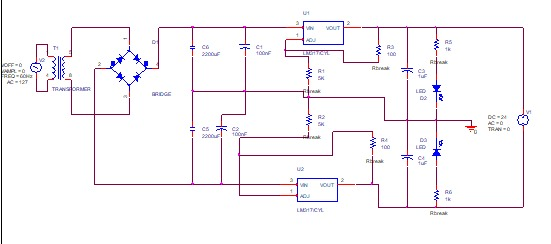
\includegraphics[width=12cm]{Fuente.jpeg}
\caption{Esquematico de la fuente de alimentacion}
\end{figure}

En el diagrama de la fuente de alimentacion regulada, se pueden ver los componentes que esta tendra, siendo el mas destacado de ello el regulador de voltaje lineal Lm317, se propuso este componente, como una estimacion de lo que otros componentes podrian tambien hacer, como lo es regular el voltaje y variarlo al valor que se ocupe (En este caso para los motores), pero esto lo estimaremos mejor ya que entremos a temas de convertidores de voltaje, en la clase de Sistemas Electronicos de Interfaz. Por esta parte adquiriendo el conocimiento suficiente para poder establecer un mejor componente, o un mejor acomodo del esquematico,para mejoras e innovaciones que podria tener el sintetizar este tipo de fuentes para el uso en el trabajo mecanico, en cuestion de potencia. En este se toma en cuenta que el voltaje minimo que puede manejar son 1,25v a 100mA, especificaciones que son de ayuda.

\section{Calculos:}
En seccion al calculo del brazo robotico. Para poder empezar con el caluclo dinamico de este brazo robotico, en constancia de previsualizacion a una estimacion dada hipotesis en perpectiva a los materiales y a la resistencia que tendran estos, para el movimiento, carga y distribucion de peso de este, Siendo este caso, mas simplificado, para no atraer problemas a la hora del armado que tenga este y sus piezas.\\

Caracteristicas del brazo:\\
Altura: 40 cm apoximadamente.\\
Peso: 8Kg aproximadamente.\\
Caracteristicas del motor:\\
Voltaje dc: 6v-24v.\\
Corriente: 1.10 A.\\
Revoluciones: 10,000rpm.\\
Diametro del motor: 36mm.\\
Diametro del torque: 3.17mm.\\
Con esas caracteristicas, se puede dar una idea, de como quedaria establecido la dinamica del brazo robotico, en este caso, viendo mas que nada factores como los motores, o el peso que cargara el brazo y en estancia con que esfuerzo.\\
Se calcula de primera estancia el trabajo de los motores, estabeciendo el trabajo de estos:\\

Establecemos el punto de partida de la posicion en la que se encontara al momento del giro del motor:\\

$$ \emptyset=\frac{4mm}{3.17mm}= 1.3mm $$

En constancia al centro del diametro, el momento en que se mueve este, se encontrara en 1.3mm, respectivamente en movimiento.\\
Ahora queremos cambiar de revoluciones, a radianes por segundo, para asi poder ver el movimiento en los 360°, que esta establecido el torque del motor, quedando:\\

$$ 1rev=2\pi=360°$$

$$ 10,000 \frac{vueltas}{min}*\dfrac{2\pi rad}{1 vuelta}*\frac{1 min}{60s}= 333.3 \pi rad/s $$

Simplificando \pi queda:\\

$$ 333.3 rd/s* \pi= 1,047.2 rd/s $$

Ahora teniendo datos, simplificados, para ver como trabajara en la realizacion mecanica, el motor, podremos calcular el momento, entre otros factores del brazo, para su péso en una previsualizacion.\\

$$ M= P*D $$

Simplificando datos:\\

$$ M=0.40m*8kg= 3.2 m/kg $$

Esto ayuda a la hora de carga del objeto en cuanto la garra, y el motor, simplificando el trabajo que pueda hacer tanto mecanico, como de potencia.\\
En otro punto, el centro de masas nos ayuda en este caso, a ver el estable movimiento en el que se puedan encontrar tanto el peso del brazo, como el del objeto a cargar, siendo este:\\

$$ CM=\frac{3.2 m/kg}{8kg}= 0.40m $$

Como se aprecia en el resultado, nos da el inicio del brazo, esto quiere decir que el centro de estabilidad, se encuentra al principio de este. Conceptuando la longitud que tendra el brazo, y donde tendra todo su impetu, a la hora de carga y de trabajo.\\
En otro caso, el trabajo que pueda realizar este, dejandolo con la siguiente formula:\\

$$ W= F*cos(45°)*d $$

Esta formula respectivamente del angulo es un alcance del angulo que puede tener para la liberacion de grados de libertad.\\

$$ W= 160N*cos(45°)*0.40m= 48.7 J $$

Dejandonos apreciar el trabajo que podriamos tener, en un punto del agarre. En otro factor la potencia, que se mide en este caso para la fuerza y el movimiento en le momento del agarre y traslacion del objeto que el brazo cargue, va dirigido, a caballos a vapor, que queda como una constante.

$$ 1CV= 736W= Caballo de vapor $$

Nota: Estos calculos, solo son una perpectiva, de lo que podria ayudarnos, a terminos mas complejos, como el caso de las articulaciones, y el manejo de la potencia en conjunto, siendo estos una guia de poder ver la realizacion y el armado, de los motores respecto al centro de carga y el alcance que podria tener, este brazo robotico, analizandolo mas adelante, con dinamica avanzada.\\

\textbf{Fuente de Alimentacion Variable:\\}
Los calculos de la fuente variable queda establecido en la visualizacion del esquematico:\\
La formula para la obtencion del voltaje, dadas resietncias es:\\
$$ V_{out}= 1.25v(1+\frac{R1}{R2}) $$
Obteniendo datos:\\
$$ V_{out}= 1.25v(1+\frac{3900 ohm}{220 ohm})=23.4 voltios $$
Esta primera formula sintetiza, los valores de la resietncia R1 y R2, que nos ayudan a que el flujo de la corriente sea especifico. Quedando el voltaje de salida en 23.4v.\\

$$ Vp= \frac{V_{rms}}{0.707} $$

Obteniendo datos:\\

$$ Vp=\frac{16v}{0.707}= 22.6 v $$

Esta formula obtiene los datos, del Vrms, los 16v, son los del transformador que se podria utilizar. Ahora se aprecia en el esquematico, que hay un puente de diodos, conectando dos diodos, al transfromador y los otros tanto parte negativa, como parte posityiva del Lm317 en el Vin, nos dejan un resultado de la asiguiente forma:\\

$$ V_{dc}=\frac{2(22.6v)-1.4v}{\pi}= 14 v. $$

En este calculo, se tiene en cuenta que son dos diodos los que estan trabajando sobre la misma entrada, por lo que un solo diodo tiene 0.7v, esto multiplicado por dos seria 1.4v. En otro caso el dos que mutiplica al voltaje 22.6, es la cantidad de diodos que hay en ese punto.\\
Teniendo ya los voltajes, se saca la potencia con la que trabajaremos, en este caso, entre mas potencia haya, menos ruido podra tener la regulacion del voltaje, en este caso, siendo multiplicado por dos el voltaje del transformador, nos da un resultado de 32 Vatios. Ahora si sacamos la corriente establecida en el diagrama.\\

$$ P= (V)(I)= 32vatios=(22.6v)(I) $$

Sustituyendo la formula, para encontrar la corriente se hace un despeje:\\

$$ I= \frac{32va}{22.6v}= 1.4 A $$

Este valor de corriente, establecida en todo el circuito es la indicada, para el buen torque de los motores, y el movimiento de estos.\\
Para el uso de los capacitores es bueno tener en cuenta de que valor y de que capacidad se tendran que tener, pqara establecer un mejor flujo del voltaje. En los primeros dos capacitores son electroliticos, con un valor en Faradios de 2200uF a una capacidad de 30v, esto para que el voltaje que recae en las resistencias sea bien distribuido y no se sobrecargue el condensador.\\
Los segundos, son ceramicos, esto para que el flujo de corriente y el momento de carga sea mas pura, con un valor de 100nF a una capacidad de 50v, para que administre de mejor forma la regulacion de voltaje y la tercera linea de capacitores es de 1uF a 30v, esto para lo mismo, que al momento de carga, no se desperdicie demasiado, y pueda salir el voltaje que se requiere, para el funcionamiento correcto de los motores.

\section{Diagrama de Gantt posibles Materiales y Gastos:}

\begin{center}
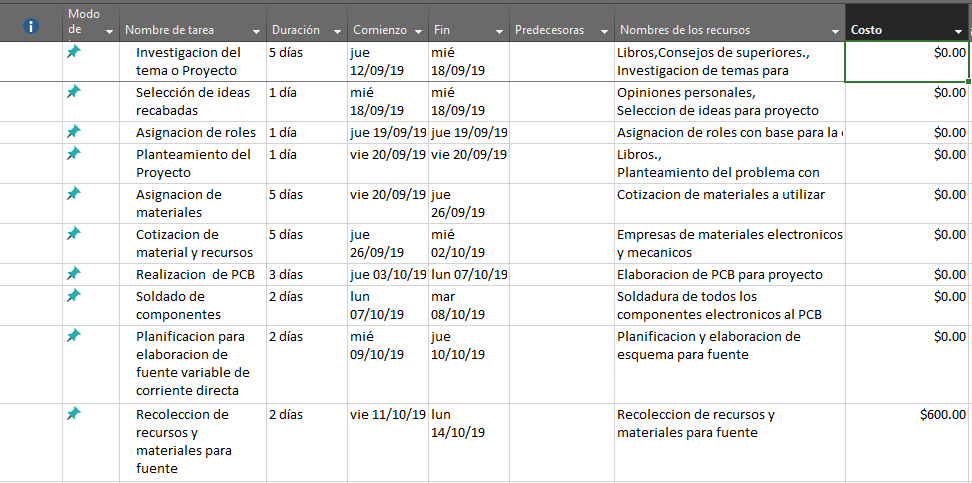
\includegraphics[width=15cm]{DefinicionTareas/4.png} 
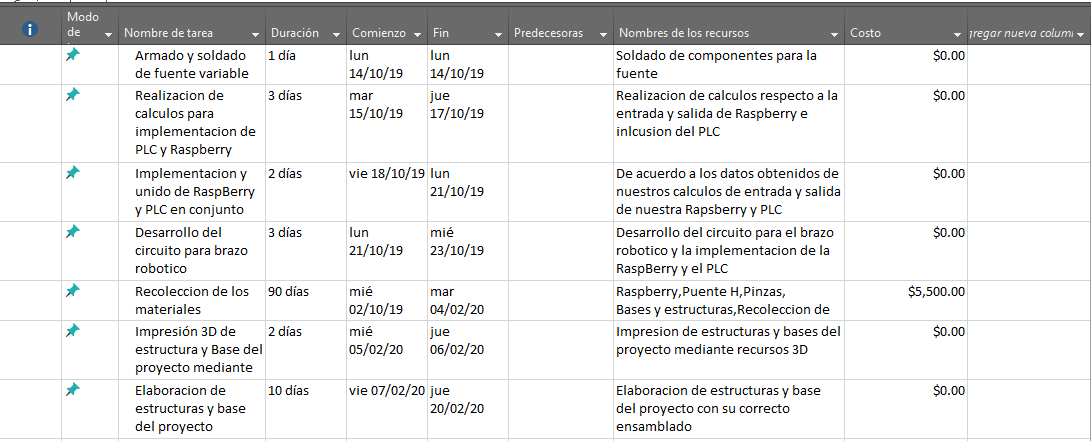
\includegraphics[width=15cm]{DefinicionTareas/5.png} 
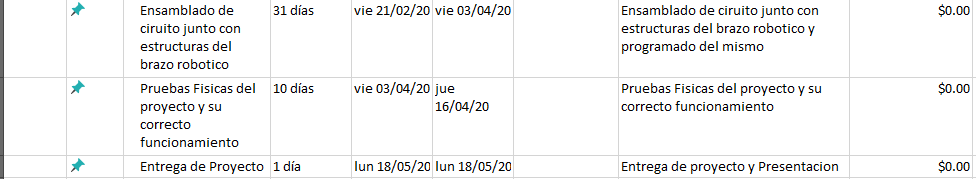
\includegraphics[width=15cm]{DefinicionTareas/6.png} 
\end{center}

\section{Diagrama de Gantt Cronograma de Actividades y Tiempo:}
Cronograma de trabajo, fechas establecidas del 12 de  Septiembre del 2019 al dia de entrega, 18 de mayo del 2020

\begin{center}

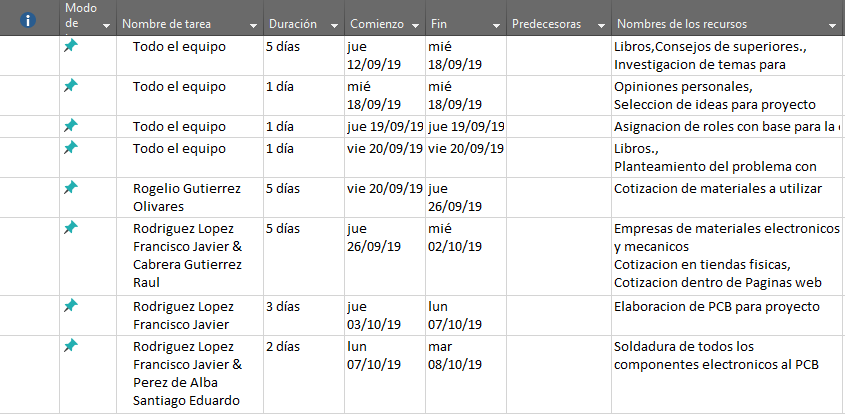
\includegraphics[width=13cm]{Esquema1.png} 
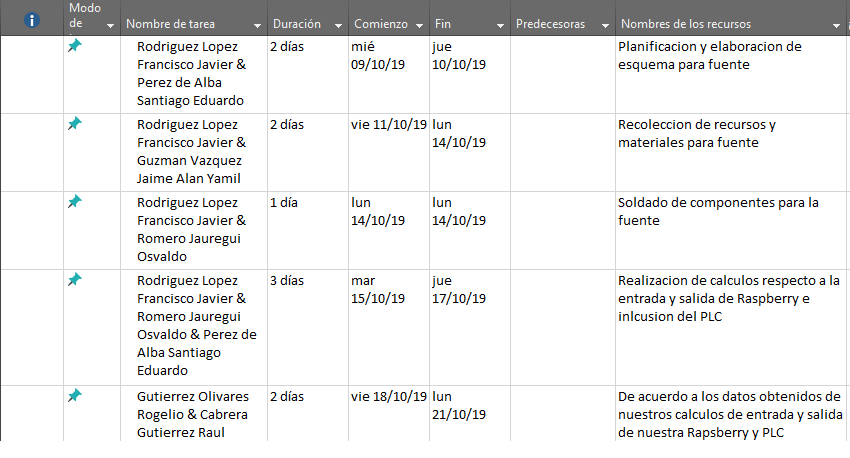
\includegraphics[width=13cm]{Esquema2.png} 
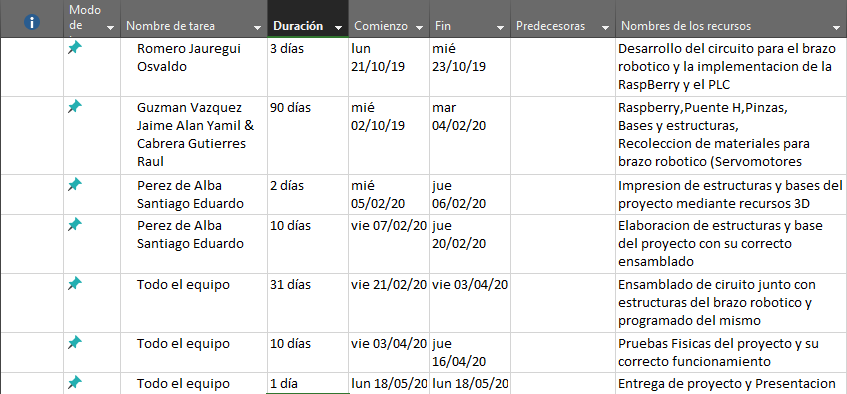
\includegraphics[width=13cm]{Esquema3.png} 

\end{center}

\section{Propuesta de Materiales:}

\subsection{Elementos consturctivos}
\begin{enumerate}

\item Manipulador o brazo mecanico.\\
\item Elementos motrices o actuadores.\\
\item Controlador.\\
\item Efector terminal.\\
\item Sensores de informacion.
\end{enumerate}

\subsection{Manipulador}
Es el conjunto de elementos mecanicos que permiten el movimiento del efector termina. En la estructura interna del manipulador se encuentran ubicador muchas veces los elementos motrices, engranajes y tranmisiones que soportan el movimiento de las cuatro partes, que por lo geneal conforman el manipulador, las cuales son \citep{puglisi2006protesis}:\\
1-Base o pedestal de fijacion.\\
2-Cuerpo.\\
3-Brazo.\\
4-Antebrazo.\\
\subsection{Elementos motrices o Actuadores}
\paragraph{Neumaticos}
Emplean aire comprimido como fuente de energia y son adecuados en el control de movimientos rapidos, pero su precision es limitada.
\paragraph{Hidraulicos}
Los actuadores hidraulicos son recomendables en los manipuladores que tiene una gran capacidad de carga, junto a una precisa regulacion de velocidad.
\paragraph{Electricos}
Los motores electricos son los mas utilizados, gracias a su precision y la facilidad de control.
\subsection{Controlador}
Es el dispositivo encargado de regular el movimiento de todos los elementos del manipulador, y de realizar los calculos y procesado de la informacion. La complejidad del control varia segun los pramatros que se gobiernan.
\subsection{Efector Terminal}
Es la garra o herramienta que se le acopla a la muneca del manipulador, siendo el encargado de materializar el trabajo previsto por ejemplo, este puede ser una tenaza, un electroiman, o algun otro aparato. En general, y de acuerdo al tipo de aplicacion, la problematica del efector terminal radica en que este ha de posser una elevada capacidad de carga y al mismo tiempo es importante que tenga un peso y tamano reducido. Por esto, en muchas ocasiones es necesario disenar el efector terminal de acuerdo a los requerimientos de la aplicacion en que se utilizara.
\subsection{Sensores de Informacion}
Los robot inteligentes son aquellos capaces e adaptarse al ambiente y tomar decisiones en tiempo real, adecuadas para situacion. La informacion que ellos reciben les hace autoprogramables, es decir,alteran su actuar en funcion de la situacion externa, lo que los hace poseer un cierto grado de inteligencia artificial. A este respecto, las informaciones mas solicitadas por los robots son las que hacen referencia a la posicion, velocidad, aceleracion, fuerzas,pares, dimensiones y contornos de objetos, y temperatura.

\section{Presupuesto:}

\begin{tabular}{|l|l|l|l|}
\hline
	Producto & Piezas & Precio & Total\\
\hline
	Impresion 3D & 5 & 70 & 350\\

\hline
	Capacitores 33pF & 2 & 5 & 10\\
\hline
	 Circuitos integrados L293B & 2 & 15 & 30\\
\hline
	Resistencias varias & 20 & 2 & 40\\
\hline
	Diodos1N4004G & 16 & 5 & 80\\
\hline
	1 Switch & 1 & 10 & 10\\

\hline
	Fuente CA-CD & 1 & 600 & 600\\
\hline
	Push bottons & 8 & 2 & 16\\
\hline
cautin & 1 & 150 & 150\\
\hline
	Estaño & 1 & 30 & 30\\
\hline
	Multimetro & 1 & 100 & 100\\
\hline
Motores DC & 5 & 400 & 2000\\
\hline
\end{tabular}

\section{Prototipo y Simulacion:}
\begin{center}
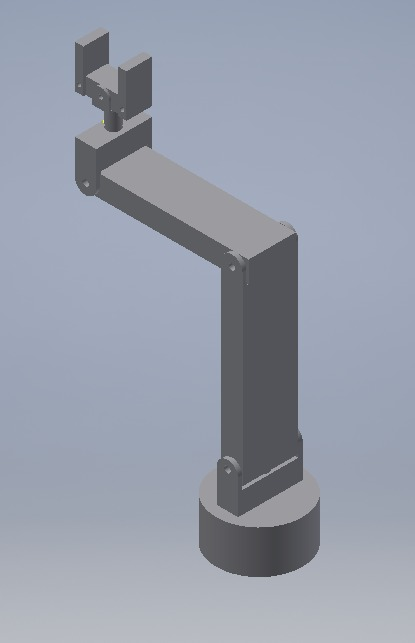
\includegraphics[width=6cm]{Proto.jpeg}
\end{center}

\begin{table}[htbp]
\begin{center}
\begin{tabular}{|l|l|}
\hline
Materia & Aportaciones \\
\hline \hline
Controladores Lógicos Programabales & \parbox{17em}{Se utilizaran microcontroladores para depurarla CPU principal de tareas sencillas } \\ \hline
Estructuras y Propiedades de los materiales & \parbox{17em}{Dara la pauta para las bases estructurales del brazo} \\ \hline
Programacion de Perifericos & \parbox{17em} {Esta materia portara con los conocimientos de programacion para el optimo control de este.} \\ \hline
Sistemas Electronicos de Interfaz & \parbox{17em} {La fuente de voltaje sera la parte ocn la que ayudara esta materia ademas del uso de componentes de alta potencia.} \\ \hline
Etica Profesional & \parbox{17em} {La etica profesional nos enseñara la importancia de las responsabilidades laborales y claridad en la muestra de los procesos empleados} \\ \hline
Ingles & \parbox{17em} {La aportacion que esta materia podria mostrar es que todos los lenguajes de programacion, datashets y programas que utilizaremos estan en el idioma ingles.} \\ \hline

\end{tabular}
\end{center}
\end{table}

Hasta este momento, con el conocimiento que hemos adquirido, dado el cuatrimestre, lo que hemos aprendido se lo hemos estado tratando de adaptar, al proyecto cabo la realizacion de este, con las ideas que se vayan generando dependiendo el grado en el que se vaya, hablando por las materias, y sus planes de estudio.

\section{Aportacion a cada Materia:}

\begin{table}[h]
\centering
\scalebox{0.9}{
\begin{tabular}{|l|p{10cm}|}
\hline
\textbf{Materias de 4to} & \textbf{Detalles de la aportación al proyecto }\\
\hline 
INGLÉS IV & En este tema se estará tocando temas como la programación que viene sustentada en ingles, así como el reporte final \\ 
\hline 
ÉTICA PROFESIONAL & Cumpliendo las normas que se rigen en  la creación de cualquier robot siendo sensatos de lo que estamos realizando y en que situación lo hacemos. \\ 
\hline 
ESTRUCTURA Y PROPIEDADES
\\
DE LOS MATERIALES & Viendo la duración y la buena presentación que cada material que complementa el dispositivo siendo mayor eficaz, y de utilización mas optima. \\ 
\hline 
PROGRAMACIÓN DE PERIFÉRICOS & Implementando un programa en la web, el cual deje manejar el avance de este dispositivo, a partir de comandos y compilaciones de datos almacenados en el dispositivo \\ 
\hline 
SISTEMAS ELECTRÓNICOS DE INTERFAZ & Implementando una fuente de voltaje CA-CD, el cual deje manejar con mayor eficiencia este dispositivo, complementado con diodos rectificadores, y rectificación el cual haga manejar el voltaje que se requiere \\ 
\hline 
CONTROLADORES LÓGICOS 
PROGRAMABLES & En este se estará viendo todo el control que tendrá el dispositivo en base, ya sea desde el movimiento y la implementación de cada componente para que este sea de mayor sensatez de rigidez, y pueda tener el manejo mas eficiente, manejado desde la terminal, y con sus componentes en conjunto. \\ 
\hline 
\end{tabular} 
}
\label{lineas}
\end{table}
\newpage

\bibliographystyle{plain}
\bibliography{Ref}


\end{document}